\documentclass[a4paper,12pt]{article}

% Sprach- und Zeichensatzpakete
\usepackage[utf8]{inputenc}     % Eingabecodierung UTF-8
\usepackage[ngerman]{babel}     % Deutsche Sprache
\usepackage{amsmath, amssymb}   % Mathematische Symbole

% Layout und Formatierung
\usepackage{enumitem}           % Bessere Kontrolle über Aufzählungen
\usepackage{geometry}           % Seitenränder definieren
\geometry{margin=2.5cm}

% Grafiken und Bilder
\usepackage{graphicx}           % Einbinden von Bildern
\usepackage{float}              % Platzierung von Gleitobjekten

% Hyperlinks und Farben
\usepackage{hyperref}           % Hyperlinks im Dokument
\usepackage{xcolor}             % Farben für Text und Links

% Kopf- und Fußzeile
\usepackage{fancyhdr}
\pagestyle{fancy}
\fancyhf{}
\rhead{Datensicherheit Lernzettel}
\lhead{Stand: \today}
\rfoot{Seite \thepage}

% Titel- und Abschnittsformatierung
\usepackage{titlesec}
\titleformat{\section}{\large\bfseries}{\thesection}{1em}{}
\titleformat{\subsection}{\normalsize\bfseries}{\thesubsection}{1em}{}

% Titelinformationen
\title{\textbf{Lernzettel – Datensicherheit}}
\author{}
\date{}

\begin{document}

\maketitle
\tableofcontents
\newpage

% === Abschnitt: Begriffsdefinitionen ===
\section{Begriffsdefinitionen}
\begin{itemize}
    \item \textbf{Vertraulichkeit} – Schutz vor unzulässiger Kenntnisnahme oder unbefugtem Zugriff
    \item \textbf{Integrität} – Schutz vor unzulässigen Veränderungen
    \item \textbf{Verfügbarkeit} – Nutzbarkeit von Informationen und Systemen
    \item \textbf{Authentizität} – Nachprüfbare Echtheit eines Subjekts/Objekts
    \item \textbf{Verbindlichkeit} – Handlungen können eindeutig zugeordnet werden
\end{itemize}

\vspace{0.5em}
\noindent\textbf{Übung:} Siehe Folie 10 und 18.

\vspace{1em}
\noindent\textbf{Ziel der Security:}  
Verhinderung von Bedrohungen durch Menschen oder Umwelt während des Betriebs.

\noindent\textbf{Ziel der Safety:}  
Verhinderung von Gefahren, die von technischen Systemen ausgehen.  
\textit{(Übung auf Folie 16)}

\vspace{1em}
\noindent\textbf{Kettenregel:}  
Eine Kette ist nur so stark wie ihr schwächstes Glied.  
\textit{Beispiel: In einer Passwortdatei reicht ein schwaches Passwort für einen Angriff.}

\vspace{1em}
\noindent\textbf{Typen von Angreifern:}
\begin{itemize}
    \item Innentäter
    \item Hacker
    \item \glqq Script-Kiddies\grqq
    \item Wirtschaftsspione
    \item Geheimdienste
\end{itemize}

\vspace{0.5em}
\noindent\textbf{Typen von Angriffen:}
\begin{itemize}
    \item Sniffing
    \item Spoofing
    \item Man-in-the-Middle
    \item Denial of Service (DDoS)
\end{itemize}

% === Abschnitt: Kryptologie ===
\section{Kryptologie}

\subsection{Kodierung}
\noindent Kodierung: eindeutige Zuordnung:
\[
f(x) = y
\]
Chiffrierung: mehrdeutige Zuordnung:
\[
f(x, k) = y
\]

\begin{itemize}
    \item \(x\): Klartext
    \item \(k\): Schlüssel
    \item \(y\): Chiffretext
\end{itemize}

\subsection{Verschlüsselung / Entschlüsselung}
\begin{figure}[H]
    \centering
    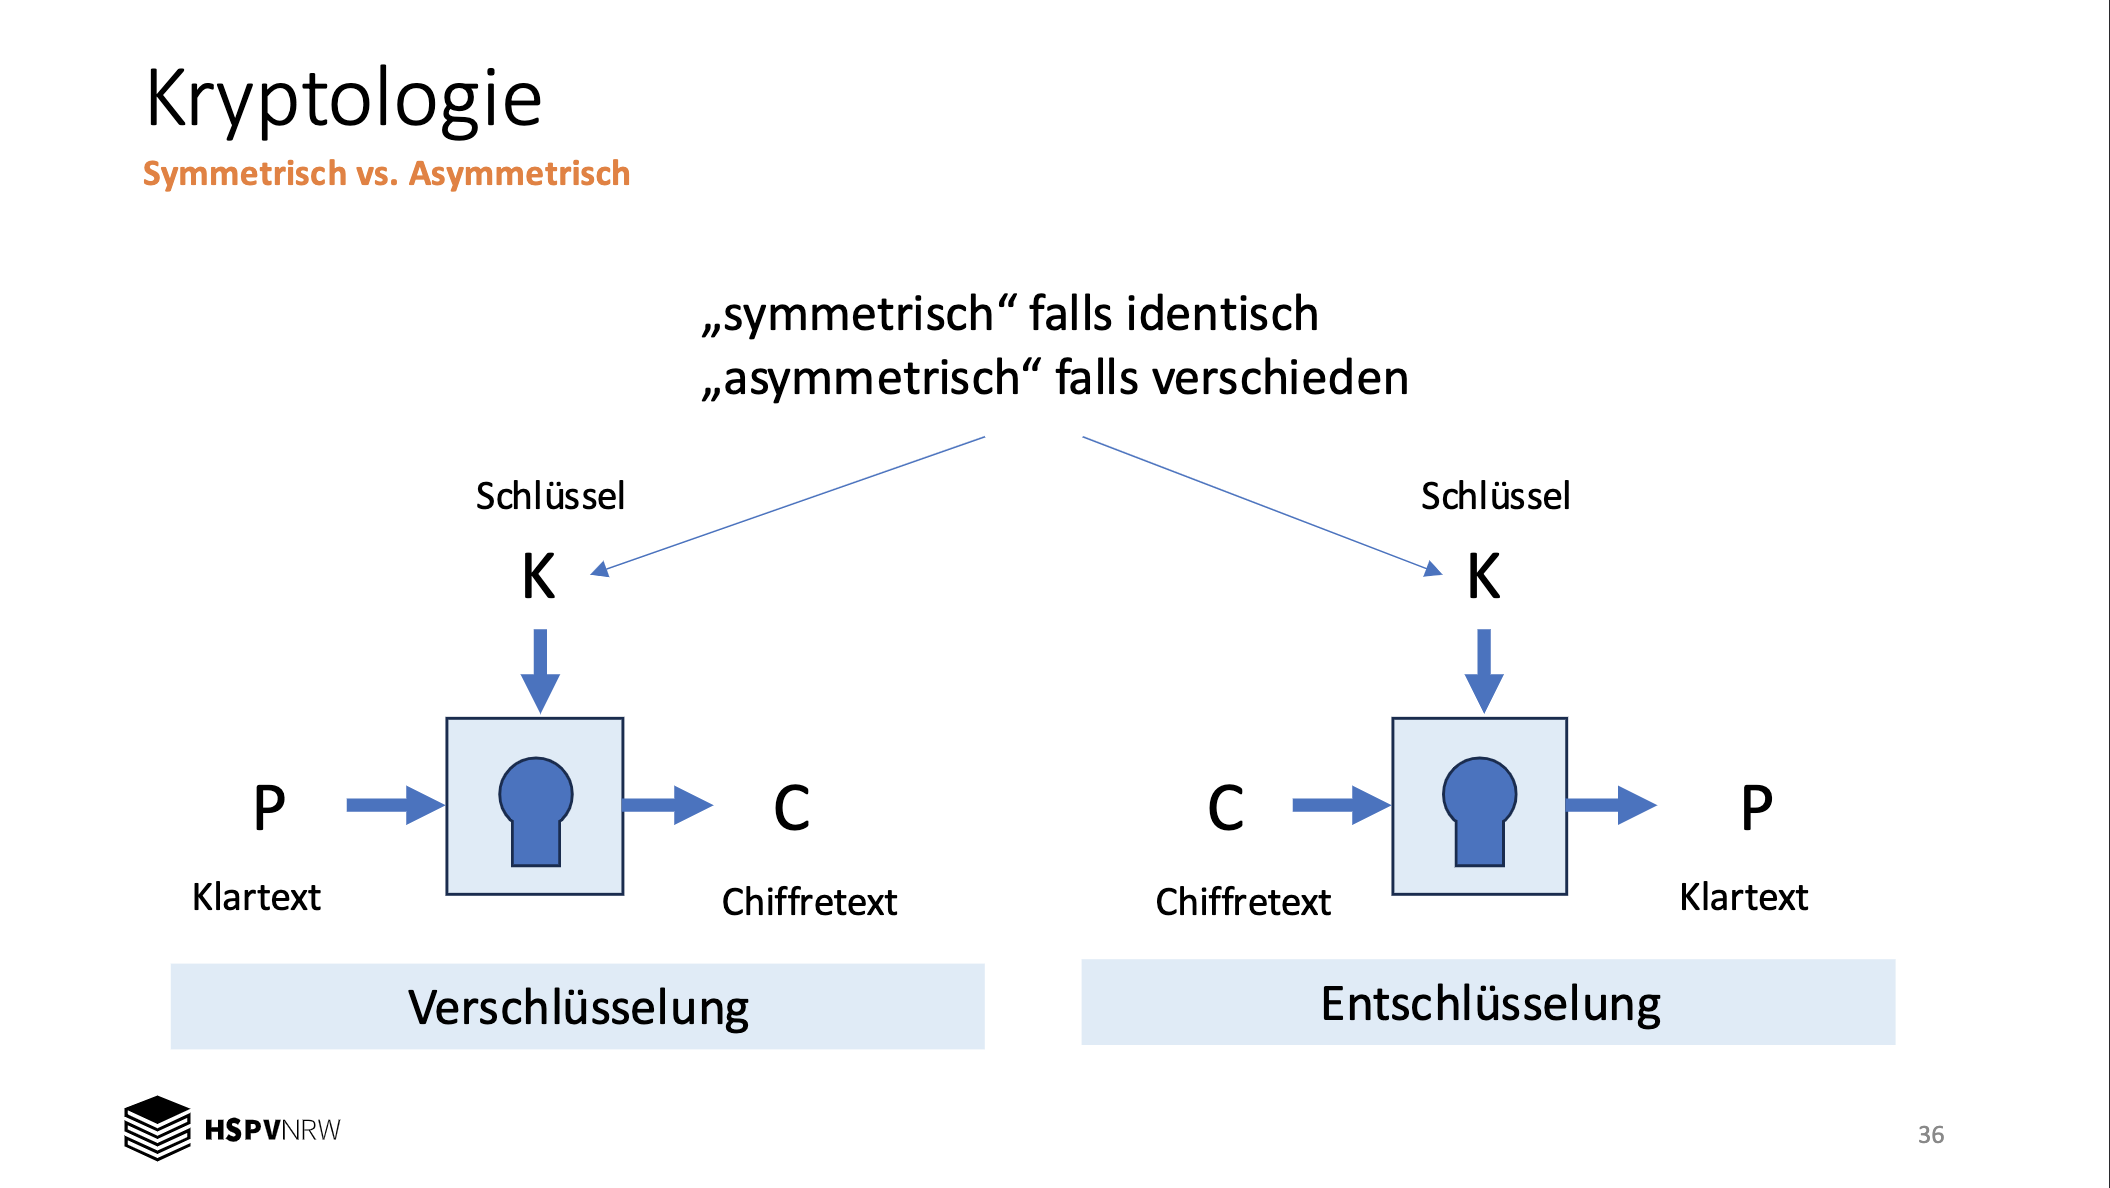
\includegraphics[width=0.8\textwidth]{bilder/verschluesselung.png}
    \caption{Verschlüsselung}
    \label{fig:encript}
\end{figure}

\subsection{Chiffren}

\subsubsection{Klassische Chiffren}
\begin{itemize}
    \item \textbf{Substitutionschiffren}
    \begin{itemize}
        \item Cäsar-Verschlüsselung
        \item Codebuch
        \item Vigenère-Verschlüsselung
        \item Playfair-Verschlüsselung
        \item \dots
    \end{itemize}
    \item \textbf{Transpositionschiffren}
    \begin{itemize}
        \item Skytale
        \item Doppelwürfel (doppelte Spaltentransposition)
        \item \dots
    \end{itemize}
\end{itemize}

\vspace{1em}
\noindent\textbf{Cäsar-Verschlüsselung:}
\begin{itemize}
    \item Verschlüsselung um 3 Stellen (z.B. A - D, B - E)
\end{itemize}

\vspace{1em}
\noindent\textbf{Playfair-Chiffre:}
\begin{figure}[H]
    \centering
    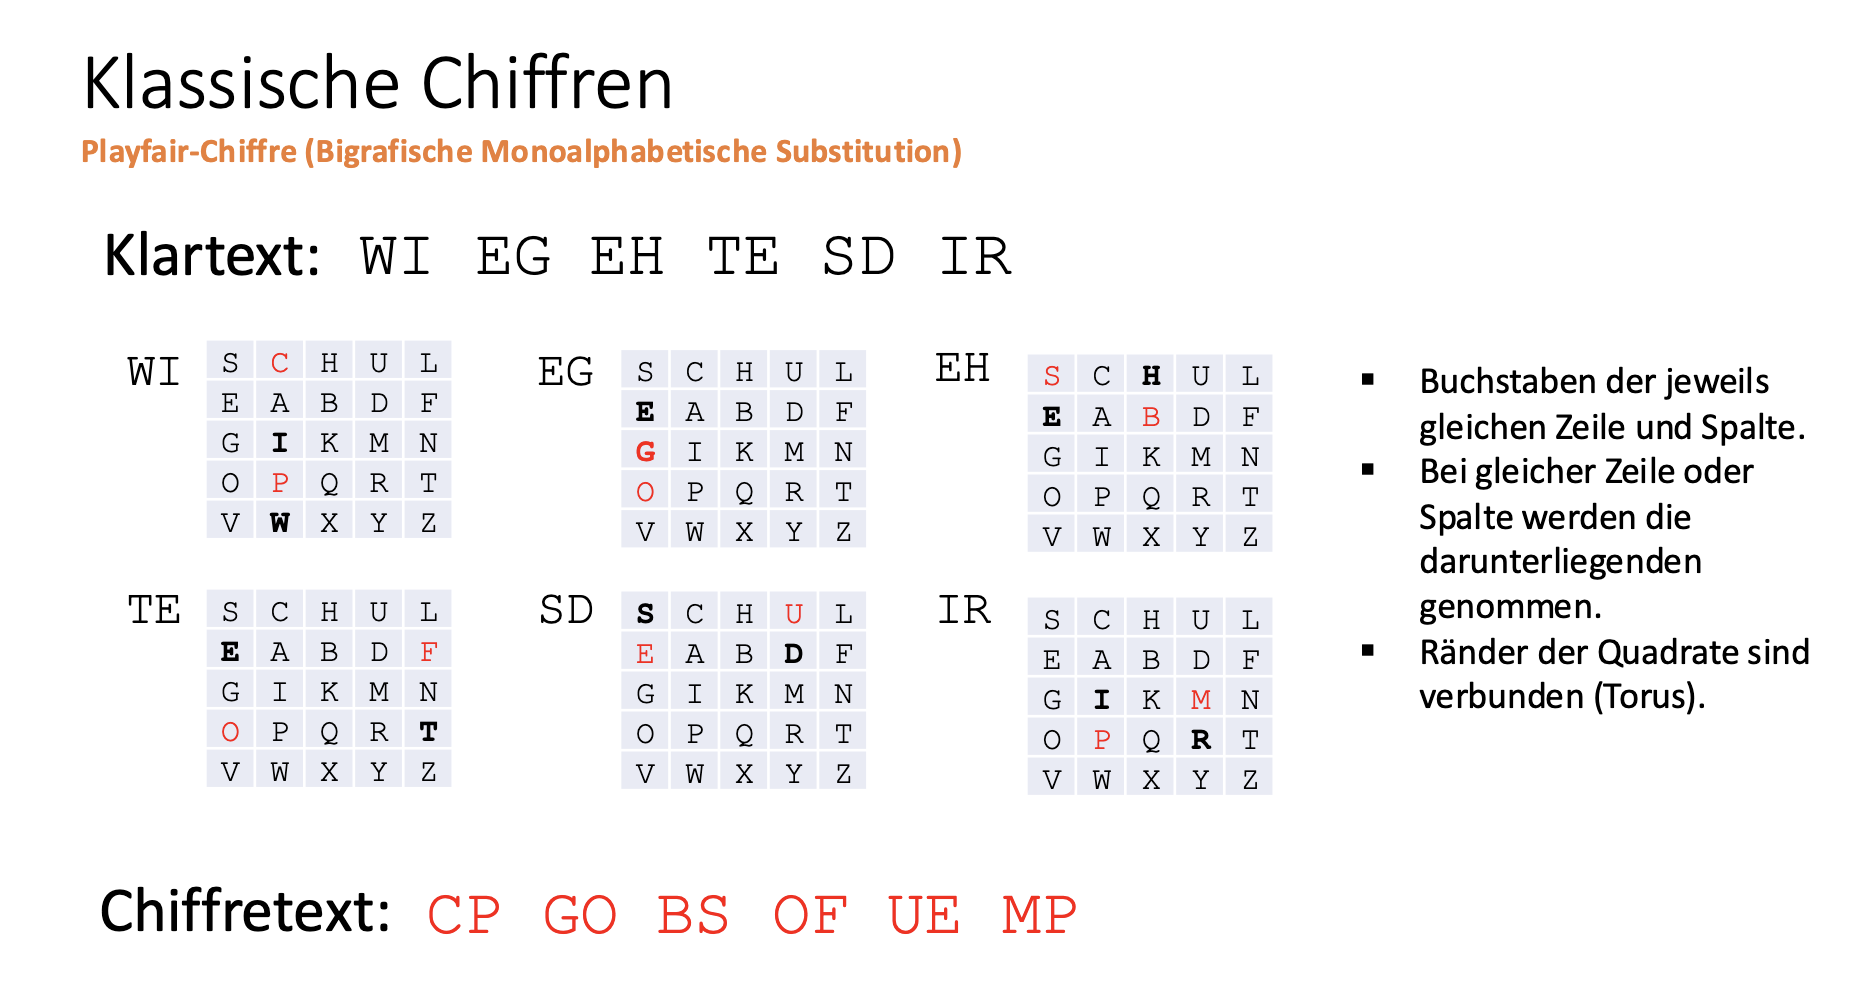
\includegraphics[width=0.8\textwidth]{bilder/playfair.png}
    \caption{Playfair-Chiffre}
    \label{fig:playfair}
\end{figure}

\vspace{1em}
\noindent\textbf{Vigenère-Chiffre:}
\begin{figure}[H]
    \centering
    \includegraphics[width=0.8\textwidth]{bilder/Vigenère-Chiffre (Polyalphabetisch).png}
    \caption{Vigenère-Chiffre (Teil 1)}
    \label{fig:vigenere1}
\end{figure}

\begin{figure}[H]
    \centering
    \includegraphics[width=0.8\textwidth]{bilder/Vigenère-Chiffre (Polyalphabetisch)2.png}
    \caption{Vigenère-Chiffre (Teil 2)}
    \label{fig:vigenere2}
\end{figure}

\vspace{1em}
\noindent\textbf{Transpositionschiffren:}
\begin{figure}[H]
    \centering
    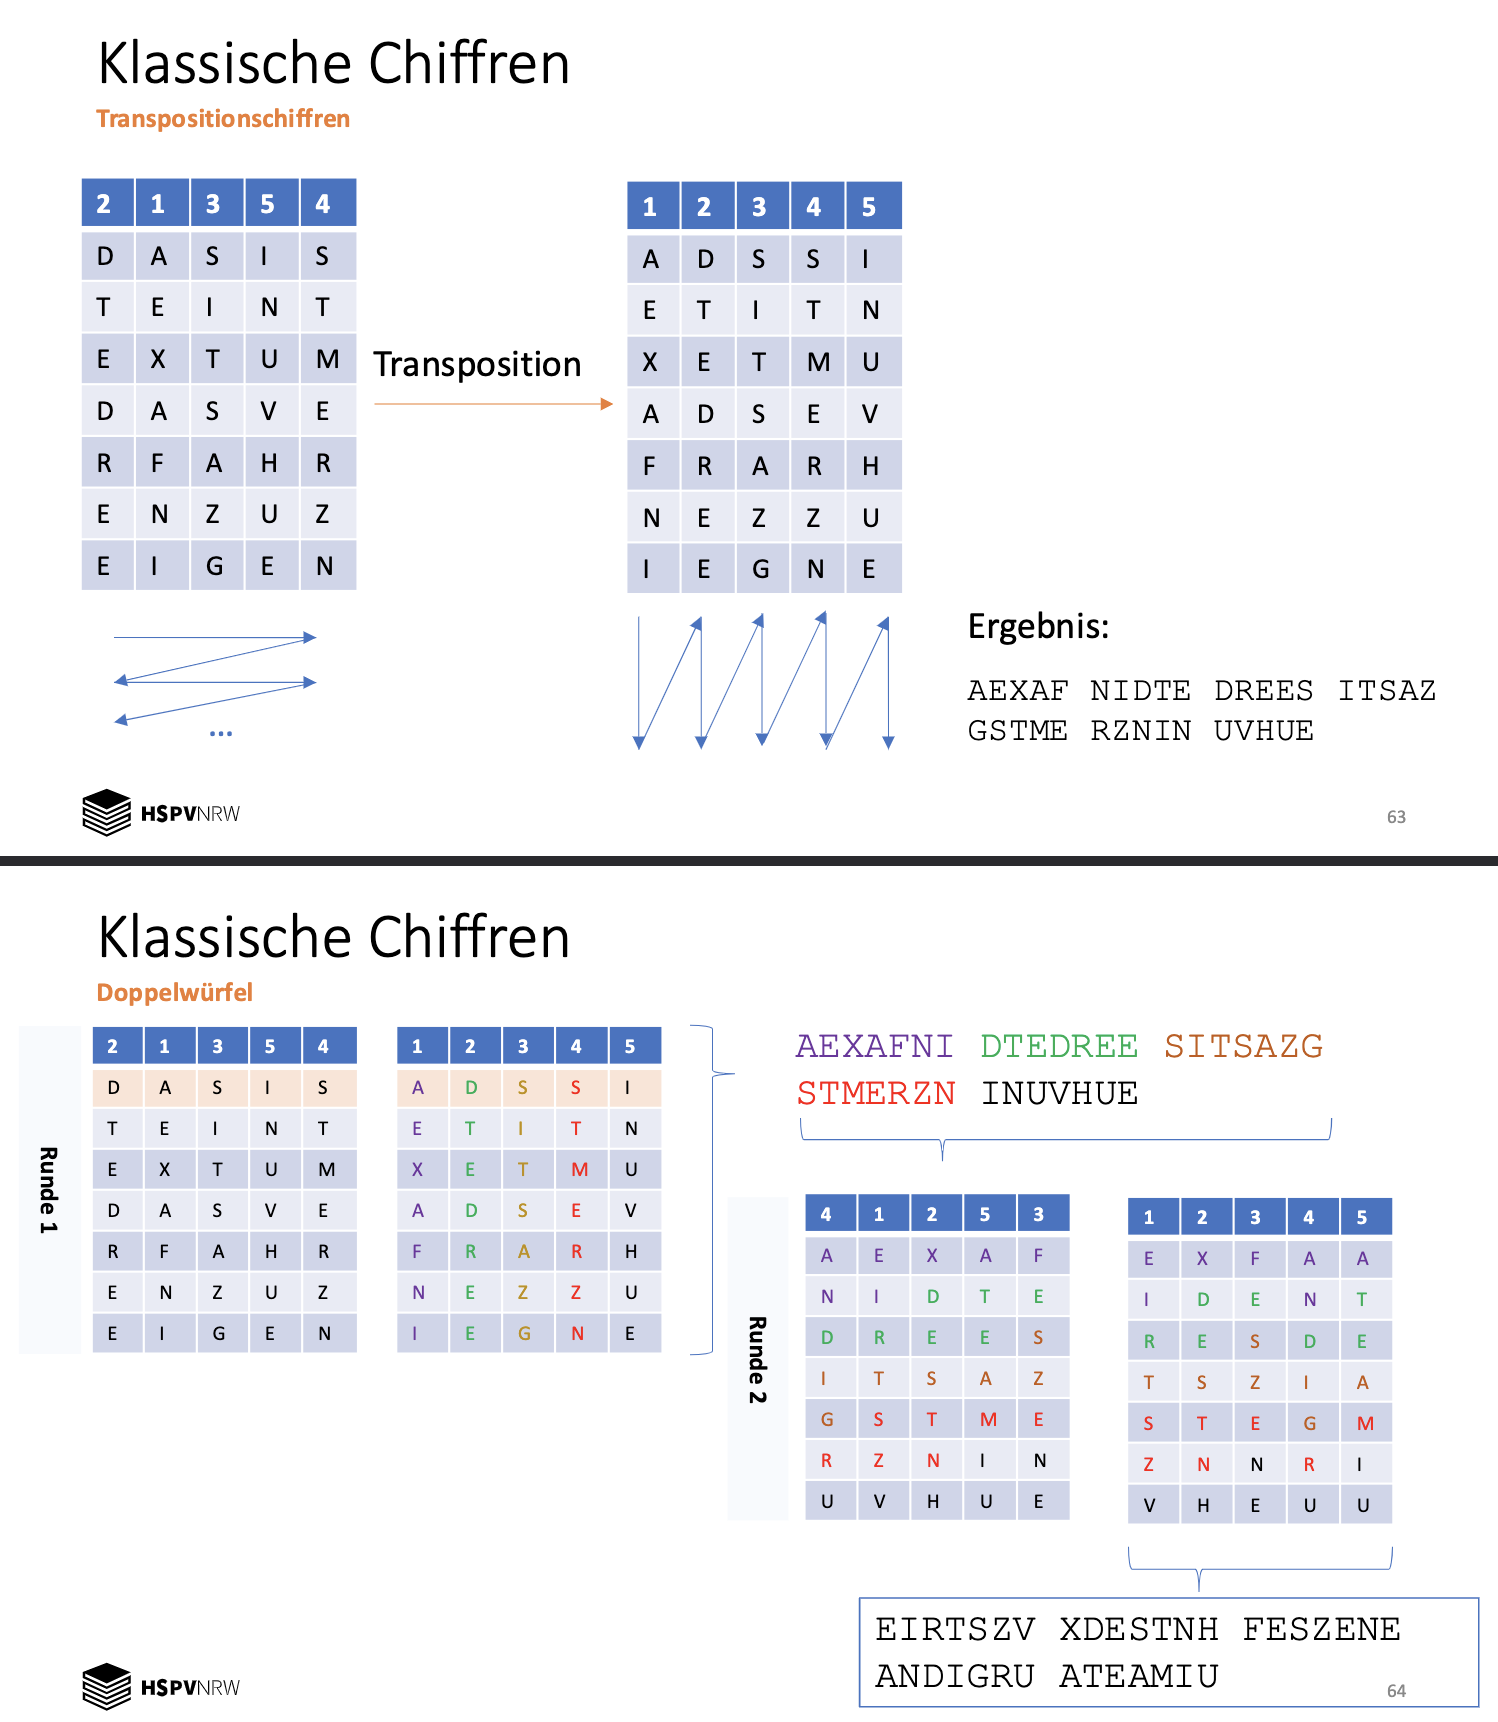
\includegraphics[width=0.8\textwidth]{bilder/Transpossitionssschiffrenn.png}
    \caption{Transpositionschiffren}
    \label{fig:transpo}
\end{figure}

\subsubsection{Moderne Chiffren – XOR-Eigenschaften}
\begin{itemize}
    \item \textbf{Kommutativität:} \quad $A \oplus B = B \oplus A$
    \item \textbf{Assoziativität:} \quad $A \oplus (B \oplus C) = (A \oplus B) \oplus C$
    \item \textbf{Neutrales Element:} \quad $A \oplus 0 = A$
    \item \textbf{Selbstinvers:} \quad $A \oplus A = 0$
\end{itemize}

\vspace{1em}
\noindent\textbf{Doppelte XOR-Verschlüsselung mit demselben Schlüssel \(K\):}
\begin{align*}
A \oplus K \oplus K 
&= (A \oplus K) \oplus K \quad &&\text{(Assoziativität)} \\
&= A \oplus (K \oplus K) \quad &&\text{(Assoziativität)} \\
&= A \oplus 0 \quad &&\text{(Selbstinvers: $K \oplus K = 0$)} \\
&= A \quad &&\text{(Neutrales Element)}
\end{align*}

\vspace{1em}
\noindent\textbf{Beispiel: HALLO}
\begin{verbatim}
H = 01001000
A = 01000001
L = 01001100
L = 01001100
O = 01001111
\end{verbatim}

\textbf{Schlüssel:}
\begin{verbatim}
11111011
00110010
11111011
10100001
11111011
\end{verbatim}

\textbf{XOR-Verknüpfung:}
\begin{verbatim}
Klartext : 01001000 01000001 01001100 01001100 01001111
Schlüssel :11111011 00110010 11111011 10100001 11111011
-------------------------------------------------------
Chiffre  : 10110011 01110011 10110111 11101101 10110100
\end{verbatim}

\textbf{Ergebnis:}  
Wendet man erneut denselben Schlüssel an, erhält man wieder den Klartext.

\vspace{1em}
\noindent\textbf{One-Time Pad:}
\begin{itemize}
    \item Schlüssel muss \textbf{zufällig} sein
    \item Schlüssel ist \textbf{nur dem Sender und Empfänger} bekannt
    \item Schlüssel ist \textbf{mindestens so lang} wie die Nachricht
    \item Schlüssel darf \textbf{nicht wiederverwendet} werden
\end{itemize}

\noindent\textbf{Stromchiffren:}

\begin{itemize}
    \item Bei einer \textbf{Stromverschlüsselung} wird auf Sender- und Empfängerseite ein identischer Schlüsselstrom erzeugt, der mithilfe der \textbf{XOR-Verknüpfung} auf den Klartext bzw. Chiffretext angewendet wird.
    
    \item Es wird ein sogenannter \textbf{Initialisierungsvektor (IV)} verwendet, um fortlaufend unterschiedliche Schlüsselströme zu erzeugen.
    \begin{itemize}
        \item Der IV wird im Klartext übertragen oder im Vorfeld ausgehandelt.
    \end{itemize}
    
    \item \textbf{Hinweis:} Die Integrität der Daten ist nicht geschützt, sofern dies nicht explizit durch das Kryptosystem vorgesehen ist.
    
    \item Bekannte Stromverschlüsselungsverfahren:
    \begin{itemize}
        \item \textbf{RC4} – heute als \textcolor{red}{unsicher} eingestuft
        \item \textbf{A5/1} – verwendet in GSM, ebenfalls \textcolor{red}{unsicher}
        \item \textbf{Salsa20}
        \item \textbf{ChaCha20}
    \end{itemize}
\end{itemize}
\vspace{1em}
\noindent\textbf{Blockchiffren:}
\begin{figure}[H]
    \centering
    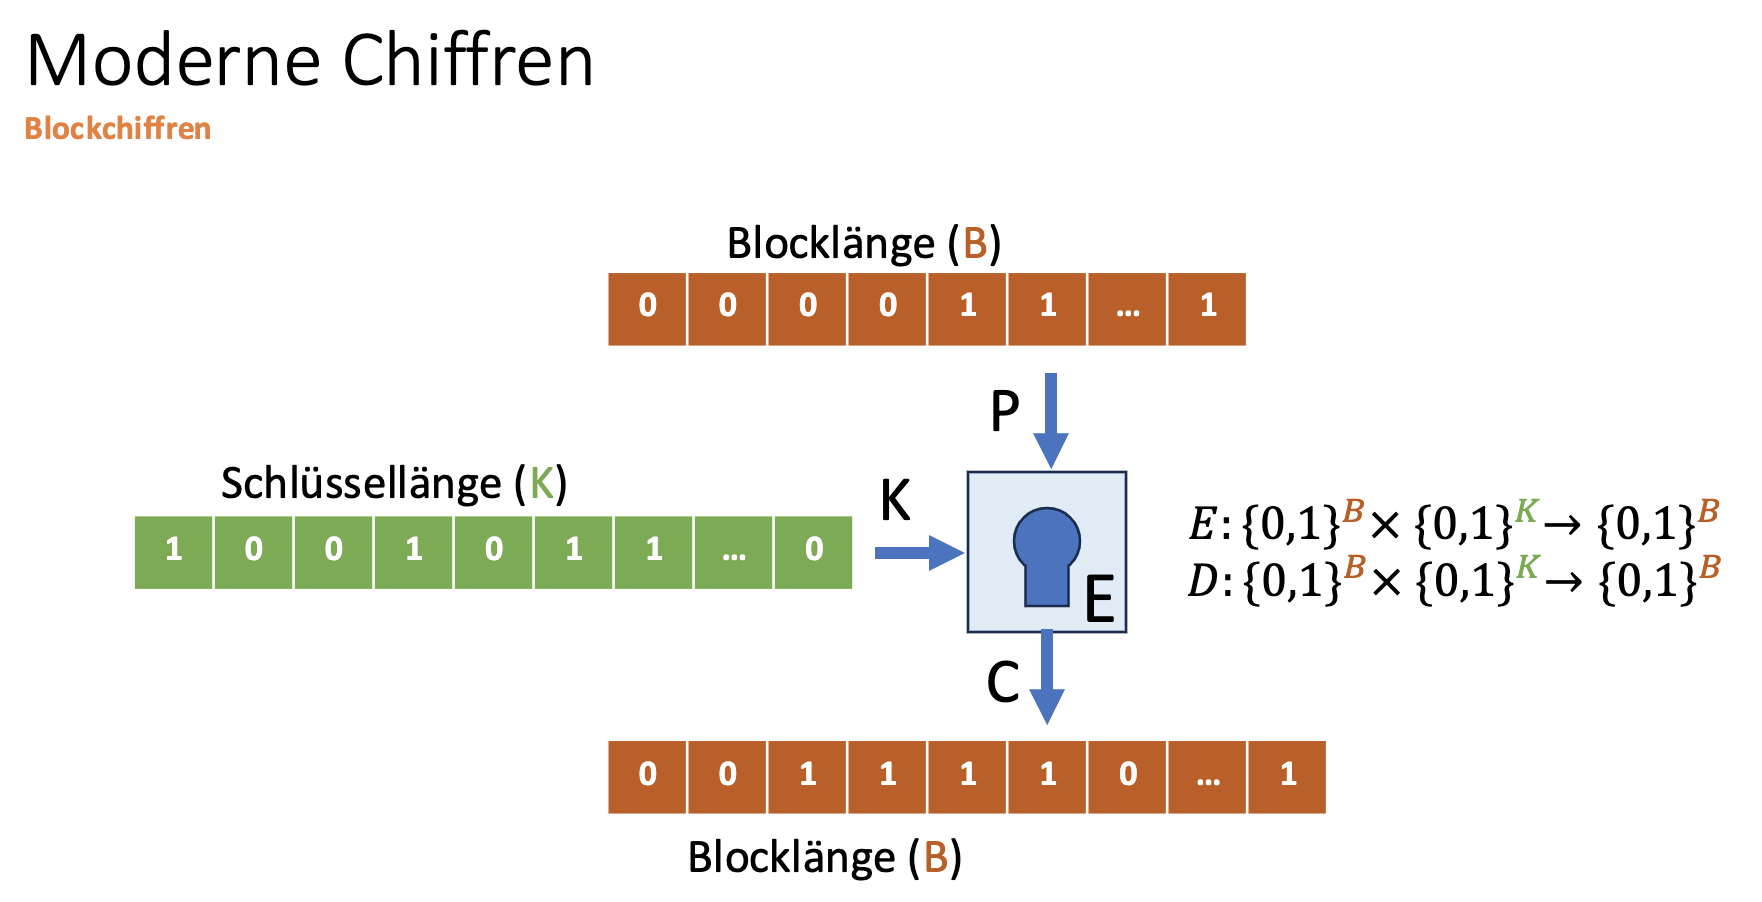
\includegraphics[width=0.8\textwidth]{bilder/blockchiffren.png}
    \caption{Blockchiffren}
    \label{fig:blockchiffren}
\end{figure}

\vspace{1em}
\noindent\textbf{AES vs. DES:}
\begin{table}[H]
    \centering
    \resizebox{\textwidth}{!}{
        \begin{tabular}{|l|l|l|}
            \hline
            \textbf{Kriterium} & \textbf{DES} & \textbf{AES} \\
            \hline
            Schlüssellänge & 64 Bit wobei 8 nicht genutzt & 128, 192 oder 256 Bit \\
            \hline
            Blockgröße & 64 Bit & 128 Bit \\
            \hline
            Struktur & Substitutionenund Permutationenin einer Feistel-Konstruktion & Substitutions-Permutations-Netzwerk \\
            \hline
            Runden & 16 & 10 (128 Bit), 12 (192 Bit), 14 (256 Bit) \\
            \hline
            Sicherheit & Als unsicher eingestuft & Derzeit als sicher eingestuft \\
            \hline
            Standardisierung & Veraltet (NIST 1977) & Aktueller Standard (NIST 2001) \\
            \hline
        \end{tabular}
    }
    \caption{Vergleich zwischen DES und AES}
    \label{tab:aes_vs_des}
\end{table}

\vspace{1em}
\noindent\textbf{Betribsmodus:}
\vspace{1em}

\noindent\textbf{ECB - Electronic Code Block}
\begin{figure}[H]
    \centering
    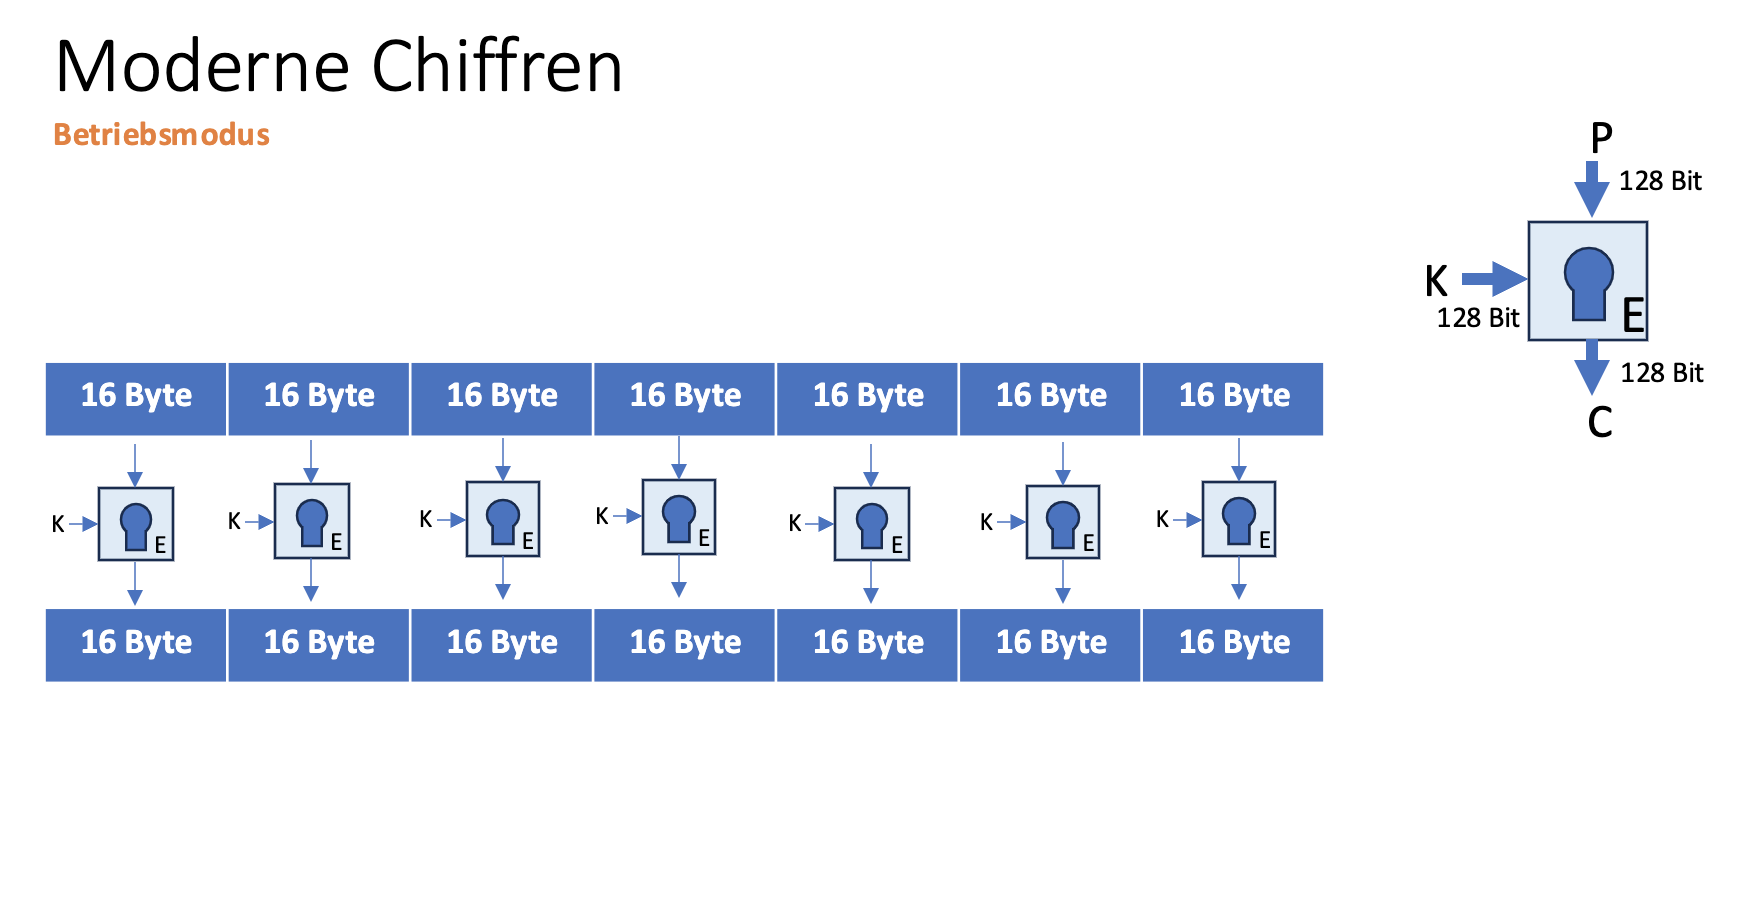
\includegraphics[width=0.8\textwidth]{bilder/ecb.png}
    \caption{ECB}
    \label{fig:ecb}
\end{figure}

\[ P = P_{1}P_{2}P_{3}P_{n}\]
\begin{itemize}
    \item Verschlüsselung: \[C_{i}=E_{k}(P_{i})\]
    \item Entschlüsselung: \[P_{i}=D_{k}(C_{i})\]
\end{itemize}
Gleiche Klartextblöcke ergeben gleiche Chiffretextblöcke.

\vspace{1em}
\noindent\textbf{CBC - Cipher Block Chaining}
\begin{figure}[H]
    \centering
    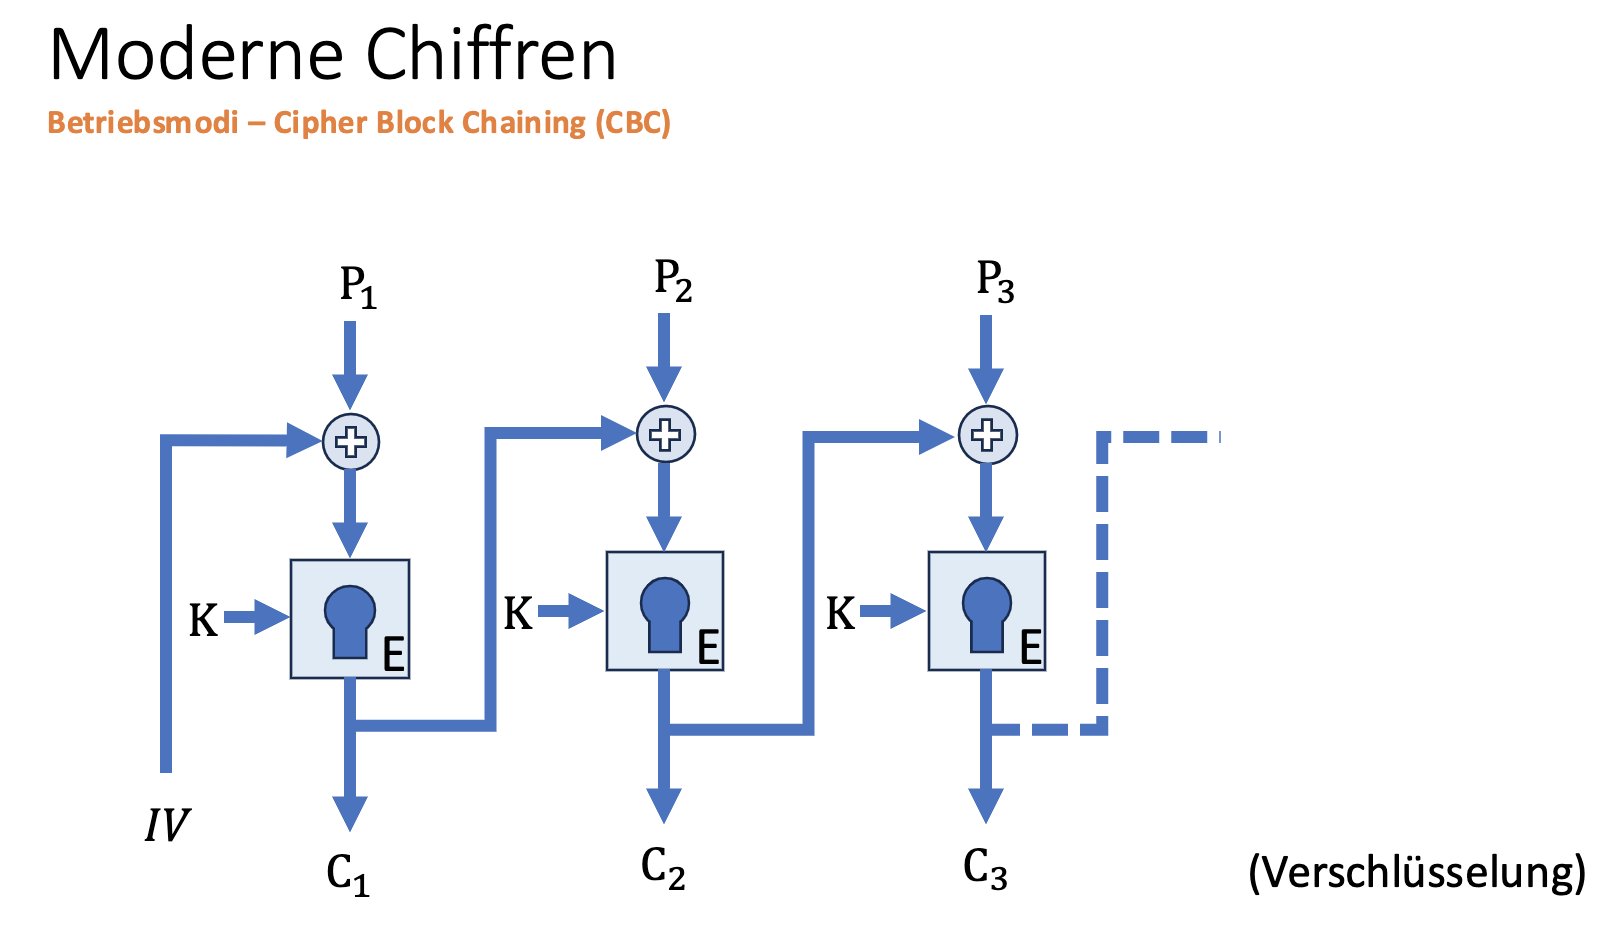
\includegraphics[width=0.8\textwidth]{bilder/cbc.png}
    \caption{CBC}
    \label{fig:cbc}
\end{figure}
\[ P = P_{1}P_{2}P_{3}P_{n}\]
\[C_{0} = IV (Initialisierungsvektor)\]
\begin{itemize}
    \item Verschlüsselung: \[C_{i}=E_{K}(C_{i-1}\oplus P_{i})\]
    \item Entschlüsselung: \[P_{i} = D_{K}(C_{i}) \oplus C_{i-1}\]
\end{itemize}
\textit{Übungen auf Folie 102}

\vspace{1em}
\noindent\textbf{OFB - Output Feedback Modus}
\begin{figure}[H]
    \centering
    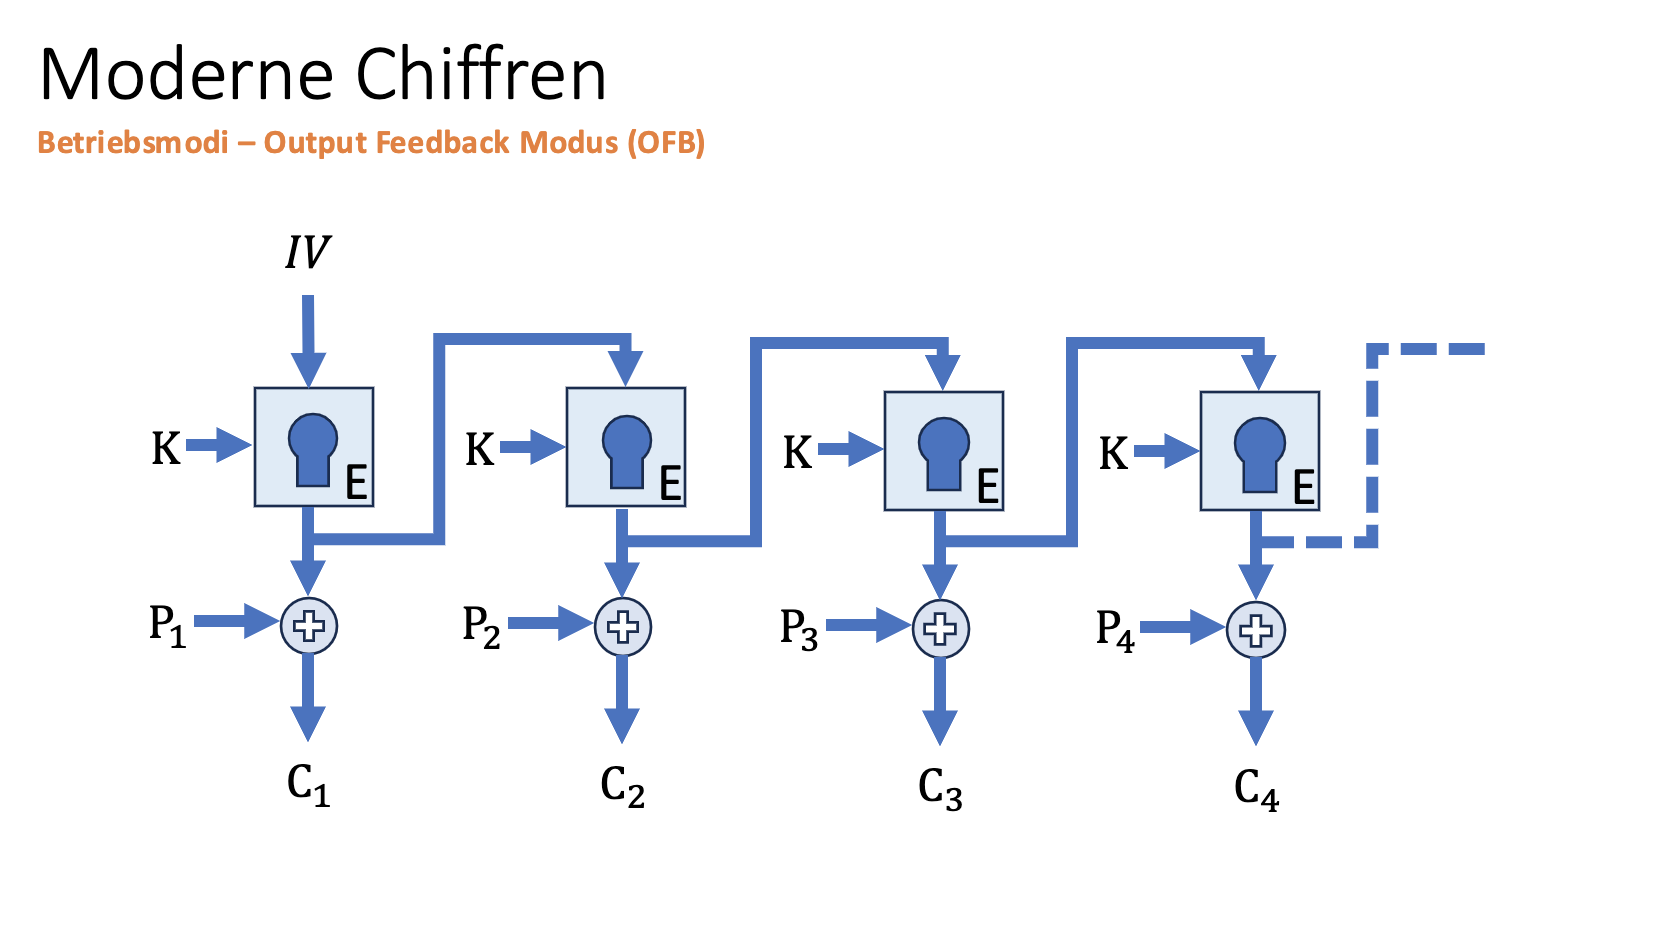
\includegraphics[width=0.8\textwidth]{bilder/ofb.png}
    \caption{OFB}
    \label{fig:ofb}
\end{figure}
\textit{nicht umbedingt Klausurrelevant}

\vspace{1em}
\noindent\textbf{CTR - Counter Modus}
\begin{figure}[H]
    \centering
    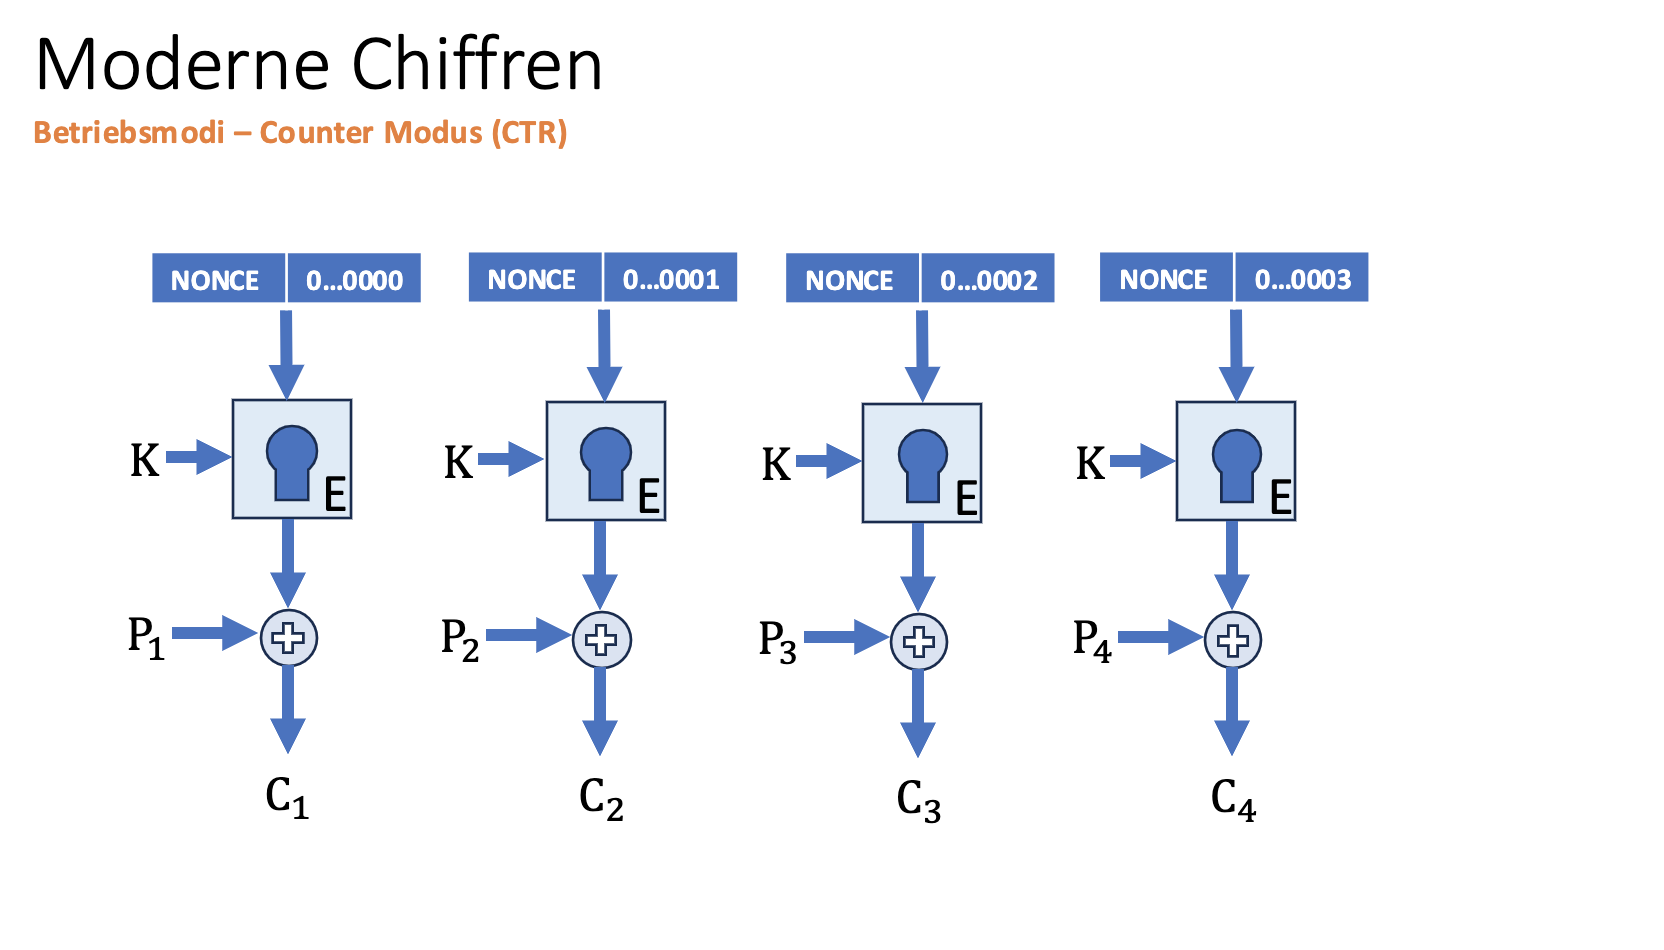
\includegraphics[width=0.8\textwidth]{bilder/ctr.png}
    \caption{CTR}
    \label{fig:ctr}
\end{figure}
\textit{nicht umbedingt Klausurrelevant}
\subsection{Asymmetrische Verfahren}
\subsubsection{RSA}
\begin{itemize}
    \item Modulares Rechnen
    \item Multiplikative Inverse
    \item Modulares Potenzieren
    \item Satz von Euler
    \item RSA Kryptosystem
\end{itemize}

\noindent\textbf{Modulares Rechen}\\
\textit{Modulo} (\%) ist definiert als die ganzzahlige Division mit Rest: 
\begin{table}[H]
    \centering
    \begin{tabular}{l|l}
        $12 \bmod 5 = 2$ & $(\text{da } 12 - (2 \cdot 5) = 2)$ \\
        $23 \bmod 4 = 3$ & $(\text{da } 23 - (5 * 4) = 3)$ \\
        $3 * 8 \bmod 7 = 3$ & $(\text{da } 24 - (3 * 7) = 3)$ \\
        $9 * 9 \bmod 2 = 1$ & $(\text{da } 81 - (40 * 2) = 1)$ \\
    \end{tabular}
\end{table}

\begin{align*}
    \text{I.} \quad &(a + b) \bmod n = ((a \bmod n) + (b \bmod n)) \bmod n \\
    \text{II.} \quad &(a \cdot b) \bmod n = ((a \bmod n) \cdot (b \bmod n)) \bmod n
    \end{align*}

    \begin{align*}
    40 + 51 \bmod 2 &= ((40 \bmod 2) + (51 \bmod 2)) \bmod 2 \\
    91 \bmod 2 &= (0 + 1) \bmod 2 = 1
    \end{align*}
    
    \begin{align*}
    999 \cdot 121 \bmod 3 &= ((999 \bmod 3) \cdot (121 \bmod 3)) \bmod 3 \\
    &= (0 \cdot 1) \bmod 3 = 0
    \end{align*}
\vspace*{1em}
\textit{Inverse:}
\begin{figure}[H]
    \centering
    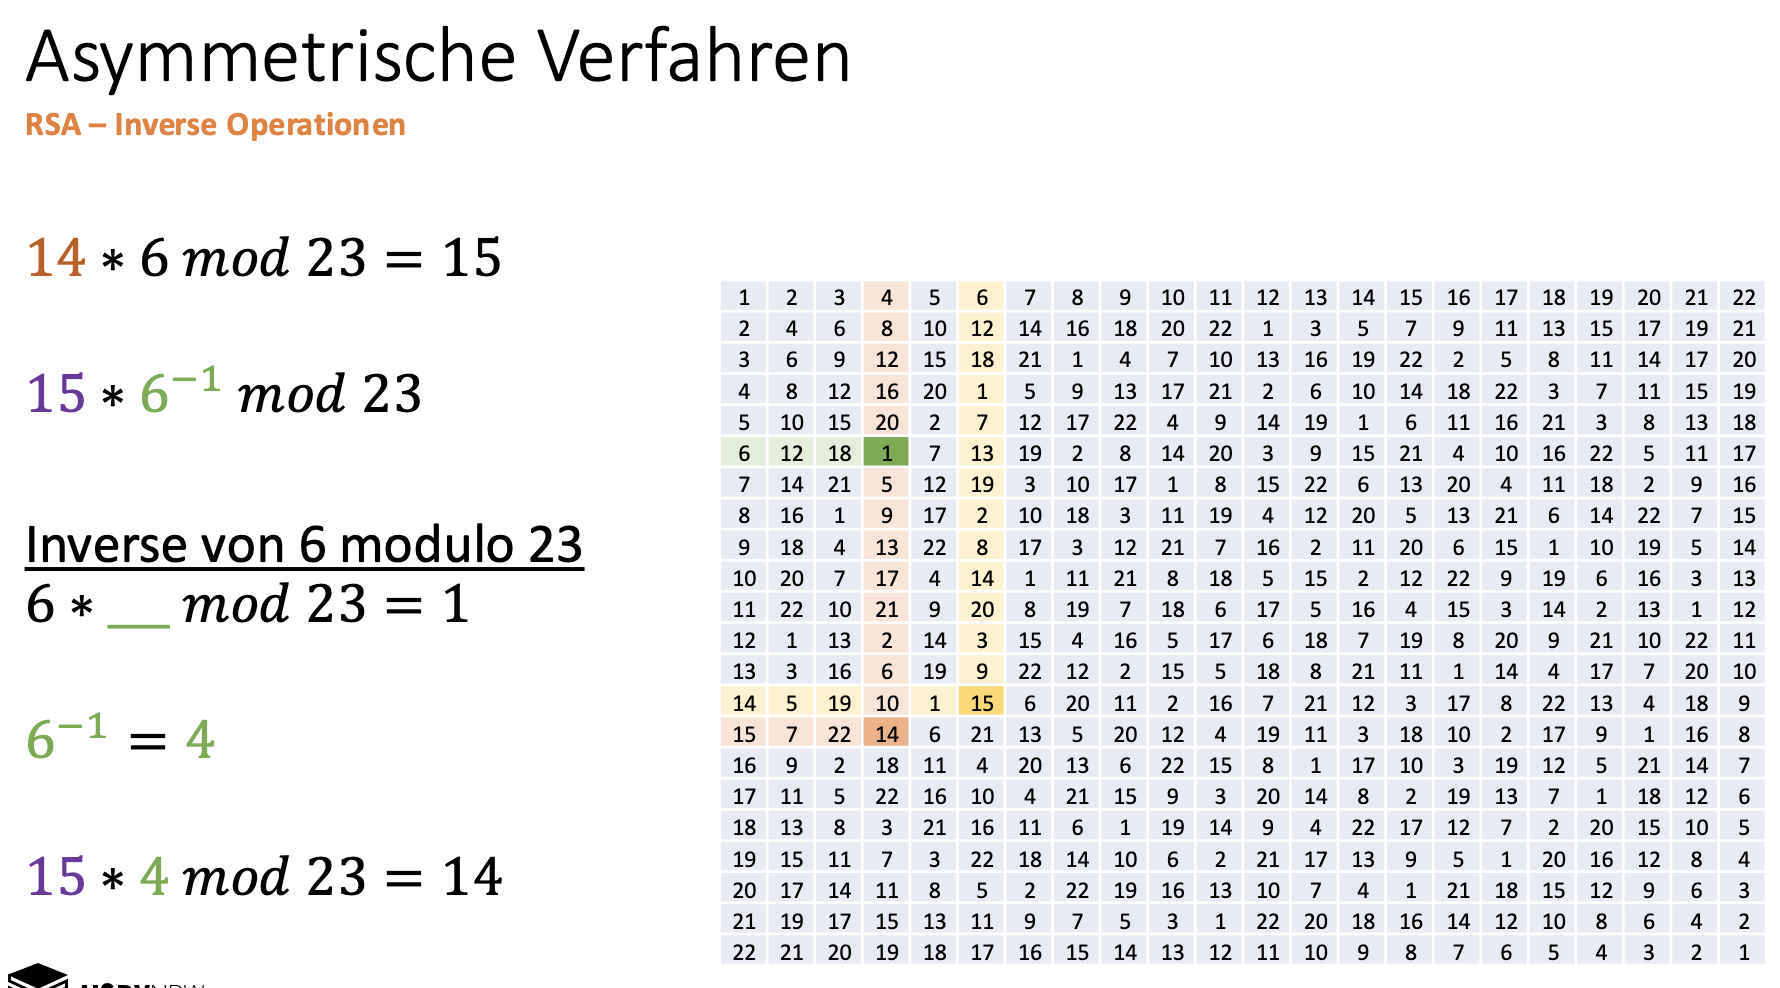
\includegraphics[width=0.8\textwidth]{bilder/inverse.png}
    \caption{Inverse - mit Multiplikationstabelle}
    \label{fig:inverse}
\end{figure}
Übunngen auf Folie 117

\vspace*{1em}
\textit{Potenzieren:}

\subsubsection{Diffie-Hellmann}

\subsection{Hashverfahren}

\subsection{Signaturverfahren}
\subsubsection{Digitale Signatur am Beispiel RSA}
\subsubsection{Hierarchiemodelle}

\end{document}